\documentclass[conference]{IEEEtran}
\usepackage[utf8]{inputenc}
\usepackage{cite}
\usepackage{amsmath,amssymb,amsfonts}
\usepackage{algorithmic}
\usepackage{graphicx}
\usepackage{textcomp}
\usepackage{xcolor}
\usepackage{blindtext}
\usepackage{hyperref}
\def\BibTeX{{\rm B\kern-.05em{\sc i\kern-.025em b}\kern-.08em
		T\kern-.1667em\lower.7ex\hbox{E}\kern-.125emX}}

\begin{document}
	
	\title{Simulating the green-beard effect with selective altruism}
	
	\author{\IEEEauthorblockN{L. Yeh}
		\IEEEauthorblockA{\textit{Faculty of Science, Utrecht University, Utrecht, The Netherlands}\\
		(Dated: \today)} 
	}
	
	\maketitle
	
	\begin{abstract}
	The green-beard effect can be simulated by having two groups of individuals. One of the groups are regular individuals, and another are individuals with a green-beard gene. An analysis of the simulations results shows that individuals with a green-beard gene have a better survival strategy than individuals without the gene. Even if the starting population size of the green-beard is significantly lower than the starting population size of the regular.
	\end{abstract}
	
	\section{Introduction}
	The green-beard effect is a hypothetical theory used in evolutionary biology to explain how altruism works among individuals \cite{hamilton1964genetical}. It is an idea coined by W.D. Hamilton, a British evolutionary biologist. Hamilton claims that altruistic behaviour can favour a species containing that trait. The name 'green-beard' stems from 'The selfish gene', a book written by R. Dawkins \cite{dawkins2017selfish}. In biology, altruism's definition refers to the action of certain individuals that aims to increase the fitness of another individual, at the cost of their own fitness \cite{barrett2008natural}. 
	
	A green-beard is an individual that has a certain 'green-beard' gene that can make other green-beards recognize each other. Green-beards are altruistic individuals, meaning that they will aim to help each other even if the action will make them lose fitness \cite{gardner2010greenbeards}. Hamilton argues that bearers of the green-beard gene are favoured by natural selection. This implies that the reproductive family members of the green-beard gene have a better chance of survival than those who do not.
	
	Although the green-beard effect started off as a hypothetical theory, there are instances of the green-beard effect taking place in the real world. Red imported fire ants is a species that contains a gene that can recognize the queens of a colony \cite{keller1998selfish}. The worker ants are able to recognize whether their queen is a polygyne colony queen (meaning that the colony has multiple queens) or a monogyne colony queen (meaning that the colony has a single queen). If a monogyne colony queen is introduced to a polygyne colony, the workers of the polygyne colony will recognize that the queen is of a monogyne colony by the body odor of the queen, and will aim to kill the queen.
	
	\section{Methods}
	The experiment aims to discover the effect of selective altruism by using individuals with and without a green-beard gene. This is done by simulating a world consisting of two species. One with the green-beard gene, called green-beards. The other without the green-beard gene, called regulars. These species will each have to find food. If they are able to find food, they will survive one generation and thus, reproduce offspring. Those who do not find food will die and will not be able to reproduce. Due to the altruistic behaviour of green-beards, the green-beards are able to share their food with other green-beards. If the green-beard has found extra food, the green-beard can share it's food with another. 
	
	Every individual has the same chance of finding food. The amount of food is equal to the population size. However, only green-beards are able to share their food.
	
	One simulation $S$ consists of a set amount of generations $G$. One simulation starts off with a starting population size of green-beards and regulars. This will count as generation 0. 
	
	One generation $G$ consists of the following processes; Starting off with the food gathering phase. The set amount of food (which is equal to the total population size) will be distributed between the entire population by randomness. Each piece of food will be assigned to a random individual of the entire population. This means that some individuals will thus have more food than others, some will have none. After the food gathering phase, the altruistic phase will start. Green-beards who have gotten more than one piece of food will share the extra food they have with other green-beards that have found none, until they have one piece left which will be kept for themselves. Due to regulars not having altruism, nothing will happen to them during this phase. After the altruistic phase, the elimination phase will start. This phase decides which individuals will live or die. The ones who have food live, but will lose their food. The ones who do not have food will be eliminated. And at last, the reproduction phase. Individuals will reproduce at the end of the generation with a 1-to-1 ratio. These phases mark one generation and the cycle repeats.
	
	In this experiment, the species that ends up with a higher population size  will be considered the one with the better strategy. The species with a higher population size $p$ will be the one who is able to adapt the best to the world, which is the definition of natural selection \cite{fisher1958genetical}.
	
	\section{Results}
	Running the simulation can give us various results depending on the parameters. The amount of simulations have been run for $S = 500$, and generations $G = 150$. The model has run with a population size of 1000 regulars $p_r$ and 1000 green-beards $p_g$. The figures showcase the average population size over the amount of simulations $S$. Figure \ref{fig:50-50} shows that the more generations that follow, the $p_g$ increases, whilst the population $p_r$ decreases. This implies that the green-beards are better at survival than regulars. 

	\begin{figure}[htbp]
		\centerline{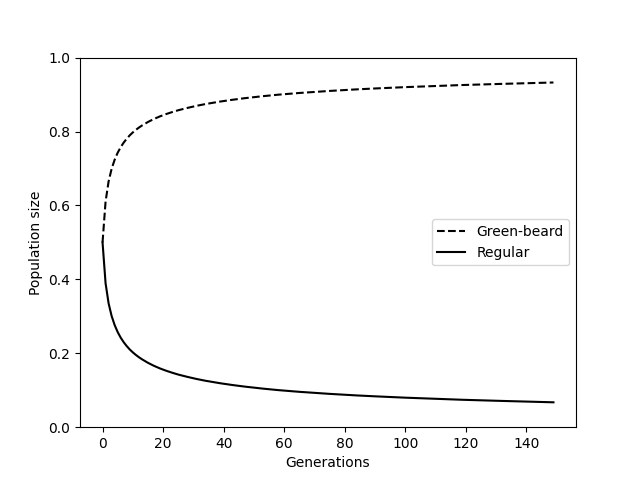
\includegraphics[scale=0.5]{figures/50-50.png}}
		\caption{Results of a simulation where the population of green-beards and regulars start off with the same population size, with starting population $p_g = 1000$ of green-beards and the starting population $p_r = 1000$ of regulars.}
		\label{fig:50-50}
	\end{figure}
	
	Running the simulation with $S = 500$ and $G = 150$ on a simulation with starting populations $p_r = 1000$ and $p_g = 500$, results the green-beards eventually taking over the regulars in terms of population size, as shown in Figure \ref{fig:1000-500}. This is true even for when the green-beards start with a lower population size.

	\begin{figure}[htbp]
		\centerline{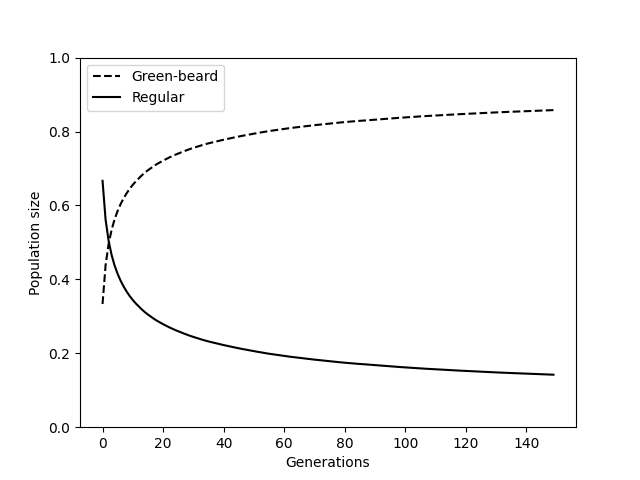
\includegraphics[scale=0.5]{figures/1000-500.png}}
		\caption{Results of a simulation where the starting population $p_g = 500$ of green-beards are significantly lower than the starting population $p_r = 1000$ of regulars.}
		\label{fig:1000-500}
	\end{figure}
	
	\section{Conclusion and Discussion}
	The results from the simulations show that individuals with the green-beard gene are better at survival than individuals who don't share that gene. In the simulations, even if the starting population of the green-beards is smaller than the starting population of the regulars, the green-beards will eventually exceed the population of regulars. This concludes that the green-beards are better at survival than regulars.
	
	Although currently only the green-beards and regulars are compared to each other, Hamilton's theory also includes two other types of individuals \cite{hamilton1964genetical}. One which is a regular who gets the benefit of green-beards, but does not contribute, and one who only gives benefit to others, but does not receive anything. In future experiments, these types of individuals can also be included in the comparison.
	
\bibliographystyle{plain}
\bibliography{references.bib}
	
\end{document}
